\documentclass{article}
\usepackage{graphicx}
\usepackage{amsmath, amssymb}
\usepackage{hyperref}
%\usepackage{cite}
\usepackage{algorithm}
\usepackage{algorithmic}
\usepackage{caption}
\usepackage{graphicx}
\graphicspath{ {./images/} }
\usepackage{booktabs} % For better table formatting
\usepackage{multirow} % For multirow cells
\usepackage{array} % For custom column alignment
\usepackage{tabularx} % For auto-adjusting table width
\usepackage{booktabs} % For better table formatting
\usepackage{adjustbox} % For scaling the table
\usepackage{geometry} % For better page margins
\usepackage{array}
\usepackage[section]{placeins} % for \FloatBarrier
\PassOptionsToPackage{hyphens}{url}\usepackage{hyperref}

\title{Analyzing Public Sentiment on Controversial Sports Events in YouTube Comments}
\date{}

\begin{document}

\maketitle

% \section{Details of Events}

\section{Samples of Comments}

We have attached the tables for a sample of annotated comments from our dataset.
\\
\noindent {\bf Table 1: } Shows examples of \textbf{Favor}, \textbf{Against}, \textbf{Neutral}, \textit{Irrelevant} from our dataset.
\\
\noindent {\bf Table 2: } Shows examples of a much detailed division of \textbf{Favor} and \textbf{Against} labels, namely, \textbf{Direct Praise}, \textbf{Direct Criticism}, \textbf{Indirect Praise}, and \textbf{Indirect Criticism}.
\\
\noindent {\bf Table 3: } Compares the number of samples of \textbf{Favor} and \textbf{Against} labels, namely, \textbf{Direct Praise}, \textbf{Direct Criticism}, \textbf{Indirect Praise}, and \textbf{Indirect Criticism}.
\\
\noindent {\bf Table 4: } Provides a statistical summary mapping detailed sub-categories to the main sentiment labels for Maradona Event.
\\
\noindent {\bf Table 5: } Provides a further statistical summary mapping detailed sub-categories to main sentiment labels for the Luis Suarez Event.
\\
\noindent {\bf Table 6: } Provides a further statistical summary mapping detailed sub-categories to main sentiment labels for the Frank Lampard Event.

\section{Logistic Classifier Performance on Model Probing}
\noindent {\bf Table 7 \& 8: } Provides a further statistical summary mapping the AUC and Accuracy scores of the trained logistic classifier on attn outputs of fine tuned and non fine tuned models.


\section{Visualisation of Probing Analysis}
\noindent { \bf {Fig 1 \& 2 \& 3} shows the same for the remaining events} 

\vspace{5mm} % Add space before table

\begin{table*}[htbp]
    \centering
    \resizebox{\textwidth}{!}{%
        \begin{tabular}{|c|p{4cm}|p{4cm}|p{4cm}|}
            \hline
            \textbf{Event} & \textbf{Favor} & \textbf{Against} & \textbf{Neutral} \\
            \hline
            \multirow{3}{*}{\textit{Frank Lampard Ghost Goal}} 
            & 1. Germans can't say anything about unsporting behavior.  & 1. The 1966 ghost goal had to be paid for. & 1. This was way more clear-cut than 1966. \\
            & 2. What a disgrace this Manuel is.  & 2. Payback for the 1966 final & 2. Inconclusive! Just couldn’t get a good angle. \\
            & 3. Could have been one of the greatest games.  & 3. Even Geoff Hurst said his goal didn’t count. & 3. I remember this game. \\
            \hline
            \multirow{3}{*}{\textit{Luis Suárez Handball}} 
            & 1. Morality always loses, and nice guys finish last.  & 1. Suárez cost Ghana the World Cup semi-final. & 1. He will never step foot in Ghana. \\
            & 2. I just love Luis Suarez with all his behaviors I don't know why.  & 2. This man was often mentally unstable. & 2. That was back then, now there’s goal-line technology. \\
            & 3. By apologizing, he would look stupid. & 3. Hand of Satan. & 3. It’s part of the game. \\
            \hline
            \multirow{3}{*}{\textit{Maradona Hand of God}} 
            & 1. Yup. Goalies s*cked these days. & 1. Errrrr! Hand of god? Cheater. & 1. When the football was football. \\
            & 2. The Real OG of all times. & 2. He makes the opponent look so stupid and clumsy. & 2. Back in the day nobody could play football, that's why he appeared to be that good. \\
            & 3. Number 15 goal is something else...my favourite. Bravo. & 3. The most cheating player in football history. & 3. You will never be able to pick one between Maradona and Messi. \\
            \hline
            \multirow{3}{*}{\textit{Jonny Bairstow Run-Out}} 
            & 1. That's not cheating, that's the way of winning.  & 1. Same old Aussies, always cheating. & 1. The lesson for the players is "pay attention." \\
            & 2. They gave Jonny ample time to stop walking out of his crease, so fair game! & 2. Australia cheating again. Who could have seen that coming? & 2. Growing up in Australia, we were taught to throw the ball at the batters' head if they left their crease like this. \\
            & 3. Jonny was too quick to get out of the crease, so it is totally a fair decision. & 3. Not cheating, just bad sportsmanship. & 3. This is just pure drama and I love it. \\
            \hline
            \multirow{3}{*}{\textit{Ashwin Mankadding}} 
            & 1. If a bowler can keep his foot inside the crease, a batsman can wait with the bat inside the crease until the ball is bowled. What's wrong with that? & 1. If you Mankadding, you should be ashamed of yourself. & 1. Ashwin merely expressed his disappointment but never wanted a wicket that way. \\
            & 2. This is out according to the rule. & 2. Not a fair runout considering sportsmanship and the spirit of the game. & 2. Whenever a batsman leaves the crease, he gets 1 to 2 ft benefits in running. \\
            & 3. Great presence of mind... genius of the game. & 3. This rule is absurd. How can you be allowed to run out someone without delivering the ball? & 3. Batters don’t do it on purpose; they walk out expecting the bowler to deliver the ball. \\
            \hline
            \multirow{3}{*}{\textit{The Underarm Incident}} 
            & 1. That time, it was legal to bowl underarm according to the rules. & 1. That was against the spirit of the game! Couldn't they just bowl a normal delivery? & 1. What were the exact rules for underarm deliveries back then? \\
            & 2. The bottom line is that there was nothing in the rules at the time saying you can't bowl underarm, so technically, nothing wrong was done. & 2. The greatest cowards in the world... None other than the Aussies. & 2. Carrying on about something decades later as if it's relevant today is the real injustice. \\
            & 3. Well, if they were allowed to do it, then fair play to them. & 3. Poor sportsmanship. & 3. Greatest highlight in cricket history, great footage. \\
            \hline
        \end{tabular}%
    }
    \caption{Examples of Favor, Against, and Neutral Comments for Controversial Events}
    \label{tab:event_comments}
\end{table*}


\begin{table}[htbp] % Changed from table* to table to prevent unnecessary spanning
    \centering
    \caption{Examples of Direct Praise, Indirect Praise, Direct Criticism, and Indirect Criticism}
    \label{tab:maradona_suarez_lampard_comments}
    \small % Reduce text size for better fit
    \renewcommand{\arraystretch}{1.1} % Slightly reduce row spacing
    \begin{adjustbox}{max width=\linewidth}
        \begin{tabular}{|c|p{3.5cm}|p{3.5cm}|p{3.5cm}|p{3.5cm}|} % Set column widths manually
            \hline
            \textbf{Event} & \textbf{Direct Praise} & \textbf{Indirect Praise} & \textbf{Direct Criticism} & \textbf{Indirect Criticism} \\
            \hline
            \multirow{3}{*}{\textit{Maradona Hand of God}} 
            & Maradona is sooo good. & 13 was simply incredible. & 3 was handball. Not a goal. A cheat. & You forgot to add the Hand of God goal. \\ 
            \cline{2-5}
            & An effervescent talent. & The legend forever. & Goal 12 looks like a huge offside. & Back when players played for the crowd, not money. \\ 
            \cline{2-5}
            & The legend forever. & Back when players played for the crowd, not money. & Cheating and poor goalkeeping. & Bro forgot aim bot on. \\ 
            \hline
            \multirow{3}{*}{\textit{Luis Suarez Handball}} 
            & Suarez is a legend... but seeing Asamoah after the match broke my heart. & I'm not a big fan of his but I respect him for keeping the ball from going in!  & Suarez crushed so many African dreams.. absolutely criminal. &Sleepless nights for a month \\ 
            \cline{2-5}
            & Suarez is a genius. & He did what he had to do for his country. & Absolute scumbag play. & Ghana would have won if it weren't for the handball. \\ 
            \cline{2-5}
            & I always that this was his karma for his biting incident with chiellini but beyond all that, he is one of the best predator in front of the goal and still is today. & Anyone would have done that though. & Suarez will forever be the biggest disgrace in modern football. & It's funny though because both Argentina and Uruguay cheated and both got what they had coming. \\ 
            \hline
            \multirow{3}{*}{\textit{Frank Lampard Ghost Goal}} 
            & They were voted the most entertaining team on FIFA.com. & It took 12 years, but Germany got their karma at last. & I hate Germany for what they did, it is so sad. & Wouldn't have made a difference; I'm English, and we would have lost anyway. Germany were by far the better team. \\ 
            \cline{2-5}
            & Wouldn't have made a difference; I'm English, and we would have lost anyway. Germany were by far the better team. & OSCAR-winning performance from football. & England defended like a bunch of girls. & With all the technology today, this would never happen now. \\ 
            \cline{2-5}
            & My idol was Frank Lampard, and I'm so happy to see, but that referee was an absolute disgrace, blind, and should go to the eye doctor. & This is the reason why FIFA needs VAR... & That's just poor by the officials... smh. & The revenge has been taken. \\ 
            \hline
        \end{tabular}
    \end{adjustbox}
\end{table}




\begin{table}[htbp]
    \centering
    \caption{Comparison of Events for Maradona, Frank Lampard, and Luis Suarez}
    \label{tab:events}
    \renewcommand{\arraystretch}{1.2} % Increase row height for better readability
    \begin{adjustbox}{max width=\linewidth} % Ensures table stays within page width
        \begin{tabular}{l c c c c c c} 
            \toprule
            \textbf{Event} & \textbf{Direct Criticism} & \textbf{Direct Praise} & \textbf{Indirect Criticism} & \textbf{Indirect Praise} & \textbf{Slang Usage} & \textbf{Racial Abuse} \\
            \midrule
            Maradona & 12 & 45 & 23 & 34 & 10 & 5 \\
            Frank Lampard & 8 & 50 & 18 & 40 & 7 & 3 \\
            Luis Suarez & 15 & 30 & 25 & 28 & 12 & 8 \\
            \bottomrule
        \end{tabular}
    \end{adjustbox}
\end{table}

\FloatBarrier % Ensures table 3 is placed before table 4

\begin{table}[htbp] % Use htbp for placement flexibility
    \centering % Center the table
    \caption{In-depth Comparison of Stance Labels against Direct/Indirect Praise and Criticism (Maradona) } % Add a caption
    \label{tab:statistical_summary} % Add a label for referencing
    \renewcommand{\arraystretch}{1.2} % Increase row spacing slightly for readability
    \begin{adjustbox}{max width=\linewidth} % Ensure the table fits within the line width
        \begin{tabular}{l c c c c} % l for first column (text), c for the rest (numbers)
            \toprule % Top rule from booktabs
            \textbf{Sub-category} & \textbf{E=0 (Favor)} & \textbf{E=1 (Against)} & \textbf{E=2 (Neutral)} & \textbf{E=3 (Irrelevant)} \\ % Header row
            \midrule % Middle rule from booktabs
            Direct Criticism (H=1)  & 0  & 18 & 0  & 0 \\
            Direct Praise (I=1)     & 38 & 0  & 0  & 0 \\
            Indirect Praise (K=1)   & 8  & 3  & 5  & 0 \\
            Indirect Criticism (J=1) & 0  & 6  & 4  & 2 \\
            Slang Use (L=1)         & 5  & 6  & 1  & 6 \\
            Racial Abuse (M=1)      & 3  & 4  & 0  & 0 \\
            \bottomrule % Bottom rule from booktabs
        \end{tabular}
    \end{adjustbox}
\end{table}

\FloatBarrier % Ensures previous table is placed before this one

\begin{table}[htbp] % Use htbp for placement flexibility
    \centering % Center the table
    \caption{In-depth Comparison of Stance Labels against Direct/Indirect Praise and Criticism (Luis Suarez) } % Add a descriptive caption
    \label{tab:statistical_summary_d} % Add a unique label for referencing
    \renewcommand{\arraystretch}{1.2} % Increase row spacing slightly for readability
    \begin{adjustbox}{max width=\linewidth} % Ensure the table fits within the line width
        \begin{tabular}{l c c c c} % l for first column (text), c for the rest (numbers)
            \toprule % Top rule from booktabs
            \textbf{Sub-category} & \textbf{D=0 (Favor)} & \textbf{D=1 (Against)} & \textbf{D=2 (Neutral)} & \textbf{D=3 (Irrelevant)} \\ % Header row
            \midrule % Middle rule from booktabs
            Direct Criticism (I=1)  & 0  & 34 & 1  & 1 \\
            Direct Praise (J=1)     & 18 & 3  & 2  & 0 \\
            Indirect Praise (L=1)   & 4  & 3  & 2  & 0 \\
            Indirect Criticism (K=1) & 1  & 8  & 6  & 1 \\
            Slang Use (M=1)         & 3  & 6  & 2  & 5 \\
            Racial Abuse (N=1)      & 0  & 5  & 0  & 2 \\
            \bottomrule % Bottom rule from booktabs
        \end{tabular}
    \end{adjustbox}
\end{table}

\FloatBarrier % Ensures previous table is placed before this one

\begin{table}[htbp] % Use htbp for placement flexibility
    \centering % Center the table
    \caption{In-depth Comparison of Stance Labels against Direct/Indirect Praise and Criticism (Frank Lampard)} % Add a descriptive caption
    \label{tab:statistical_summary_h} % Add a unique label for referencing
    \renewcommand{\arraystretch}{1.2} % Increase row spacing slightly for readability
    \begin{adjustbox}{max width=\linewidth} % Ensure the table fits within the line width
        \begin{tabular}{l c c c c} % l for first column (text), c for the rest (numbers)
            \toprule % Top rule from booktabs
            \textbf{Sub-category} & \textbf{H=0 (Favor)} & \textbf{H=1 (Against)} & \textbf{H=2 (Neutral)} & \textbf{H=3 (Irrelevant)} \\ % Header row
            \midrule % Middle rule from booktabs
            Direct Criticism (I)  & 0 & 27 & 0  & 0 \\
            Direct Praise (J)     & 7 & 0  & 0  & 0 \\
            Indirect Criticism (K) & 2 & 0  & 14 & 30 \\ % Interpreted from 201430
            Indirect Praise (L)   & 2 & 1  & 0  & 0 \\
            Slang Use (M)         & 8 & 20 & 7  & 0 \\ % Interpreted from 82070
            Racial Abuse (N)      & 0 & 0  & 0  & 0 \\
            \bottomrule % Bottom rule from booktabs
        \end{tabular}
    \end{adjustbox}
\end{table}

\clearpage


\begin{table*}[t]
    \centering
    \renewcommand{\arraystretch}{1.2} % Increase spacing between rows
    \begin{adjustbox}{width=0.95\textwidth} % Make table use 95% of text width
    \begin{tabular}{|c|c|c|c|c|c|}
        \hline
        \textbf{Event} & \textbf{Model Type} & \textbf{Accuracy} & \textbf{Top Token} & \textbf{Layer} & \textbf{AUC} \\
        \hline
        \multirow{2}{*}{\textbf{Frank Lampard}} & Fine-Tuned & 86\% & exact\_answer\_first\_token & 1-6 & 0.9993 \\
        & Not Fine-Tuned & 44.25\% & first\_answer\_token & 31 & 0.8973 \\
        \hline
        \multirow{2}{*}{\textbf{Luis Suarez}} & Fine-Tuned & 82.5\% & exact\_answer\_last\_token & 16-20 & 0.9901 \\
        & Not Fine-Tuned & 31\% & exact\_answer\_first\_token & 11, 31 & 0.8249 \\
        \hline
        \multirow{2}{*}{\textbf{Maradona}} & Fine-Tuned & 56\% & exact\_answer\_first\_token & 25 & 0.8468 \\
        & Not Fine-Tuned & 44\% & exact\_answer\_first\_token & 31 & 0.9431 \\
        \hline
    \end{tabular}
    \end{adjustbox}
    \caption{Logistic Classifier Performance Metrics across Different Events. The table shows the accuracy, most informative token positions, layers with highest performance, and AUC values for fine-tuned vs. non-fine-tuned models. Note how fine-tuned models consistently show higher accuracy and tend to focus attention on the exact answer tokens.}
    \label{tab:logistic_classifier}
\end{table*}

\vspace{15mm} % Add more space between tables

\begin{table*}[b]
    \centering
    \renewcommand{\arraystretch}{1.2} % Increase spacing between rows
    \begin{adjustbox}{width=0.95\textwidth} % Make table use 95% of text width
    \begin{tabular}{|c|c|c|p{8cm}|} % Increased the width of the last column
        \hline
        \textbf{Event} & \textbf{Model Type} & \textbf{F1 Score} & \textbf{Top 5 Accuracy Layers/Tokens} \\
        \hline
        \multirow{2}{*}{\textbf{Frank Lampard}} & Fine-Tuned & 0.96 & Layer 1-6, exact\_answer\_first\_token, Acc: 0.975 \\
        & Not Fine-Tuned & 0.916 & Layer 31, first\_answer\_token, Acc: 0.8625 \\
        \hline
        \multirow{2}{*}{\textbf{Luis Suarez}} & Fine-Tuned & 0.944 & Layers 16-20, exact\_answer\_last\_token, Acc: 0.975 \\
        & Not Fine-Tuned & 0.842 & Layer 10/14, exact\_answer\_last\_token, Acc: 0.775 \\
        \hline
        \multirow{2}{*}{\textbf{Maradona}} & Fine-Tuned & 0.773 & Layer 25, exact\_answer\_first\_token, Acc: 0.7875 \\
        & Not Fine-Tuned & 0.872 & Layer 31, exact\_answer\_first\_token, Acc: 0.875 \\
        \hline
    \end{tabular}
    \end{adjustbox}
    \caption{F1 Scores and Top 5 Accuracy Results from Probing Analysis. This table highlights the different levels of attention concentration in fine-tuned vs. non-fine-tuned models. Fine-tuned models generally have more consistent token focus across multiple layers.}
    \label{tab:f1_scores}
\end{table*}

\clearpage


% Force each image to appear on its own with a hard page break between them
\begin{figure}[p]
    \centering
    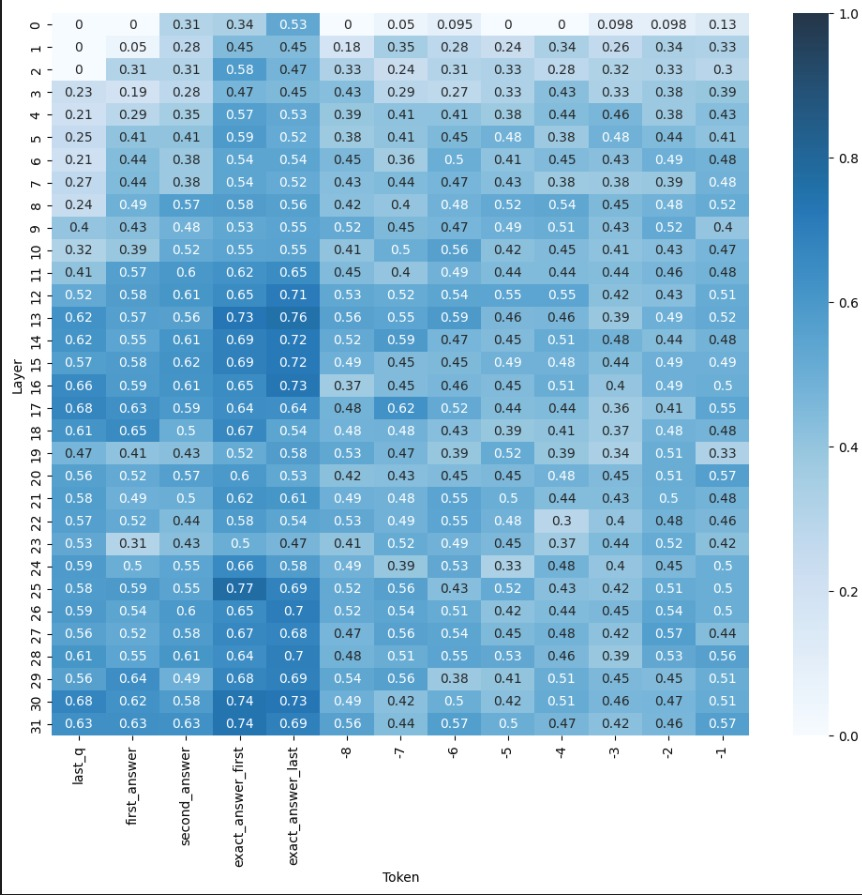
\includegraphics[width=0.7\textwidth]{maradona-positiveclass.jpg}
    \caption{Maradona Event - Positive Class}
    \label{fig:maradona-positive}
\end{figure}

\clearpage

\begin{figure}[p]
    \centering
    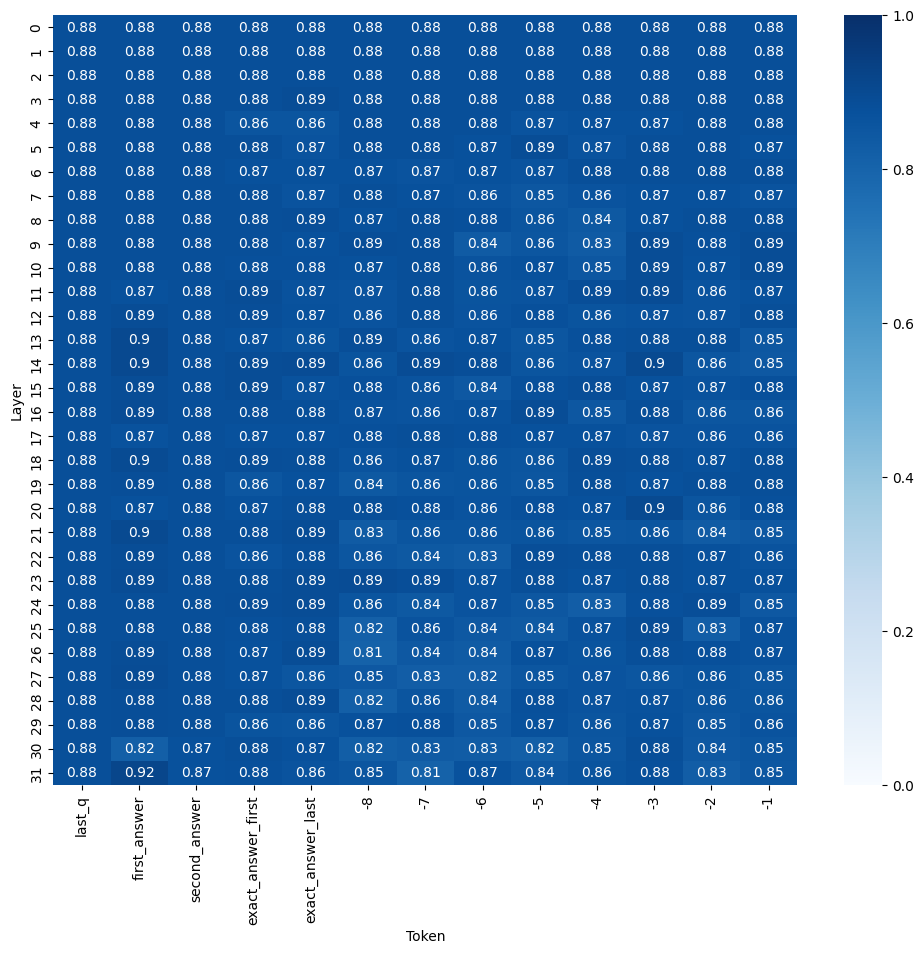
\includegraphics[width=0.7\textwidth]{frank_lampard_negative_class.png}
    \caption{Frank Lampard Event - Negative Class - diffused attention - all layers and tokens}
    \label{fig:lampard-negative}
\end{figure}

\clearpage

\begin{figure}[p]
    \centering
    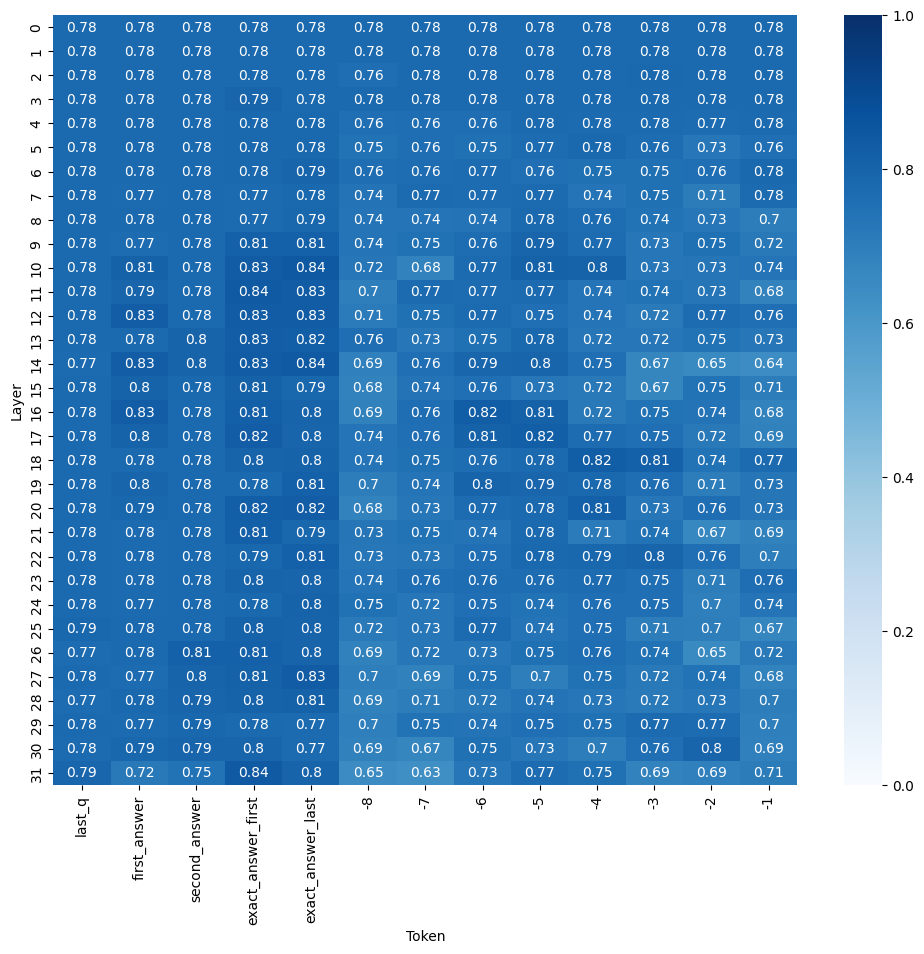
\includegraphics[width=0.7\textwidth]{luis_suarez_negative_class.png}
    \caption{Luis Suarez Event - Negative Class (diffused attention - all layers and tokens}
    \label{fig:suarez-negative}
\end{figure}

\end{document}